\chapter{Results and Evaluation}

\section{Introduction}

This chapter presents the results obtained from the AgriConnect platform and evaluates the extent to which the system fulfills the requirements defined in the analysis phase. Following the implementation described in the previous chapter, this evaluation phase aims to validate the functional behavior of the system, demonstrate its end-to-end operation through realistic interaction scenarios, and assess the contribution of each specialized agent within the multi-agent pipeline.

The evaluation is structured around three complementary perspectives. First, complete interaction scenarios are presented to illustrate how the system processes real farmer inputs from WhatsApp message reception to final response delivery. Second, each agent is individually validated through concrete input-output examples that verify its expected behavior. Third, the web application is assessed through functional testing covering the main use cases of farmers, agronomists, and administrators.

The chapter concludes with a discussion of the system's strengths and identified limitations, providing an honest assessment of the platform's current capabilities and the directions in which it could be further improved.

\section{Testing Methodology}

The evaluation of AgriConnect follows a manual, scenario-based testing approach adapted to the nature of the system. Given that the platform integrates external APIs, AI language models, automated workflows, and a web application, the testing strategy is organized around three levels of validation: agent-level unit testing, end-to-end integration testing through realistic interaction scenarios, and functional testing of the web application interfaces.

At the agent level, each specialized agent is tested independently by providing controlled inputs and verifying that the structured output conforms to the expected JSON schema and contains semantically correct content. This approach allows the behavior of each agent to be assessed in isolation before evaluating the overall pipeline.

At the integration level, complete farmer interaction scenarios are executed through the live system, covering the full pipeline from WhatsApp message reception to response delivery. These scenarios are designed to trigger different combinations of agents and to verify that the orchestrator correctly activates the appropriate sub-agents based on the input content.

At the web application level, functional testing is performed manually for each user role. A set of key use cases is executed and the result is recorded as passed or failed based on whether the expected behavior is observed in the interface and reflected in the database.

This combined approach provides sufficient coverage to validate the system's core functionalities while remaining consistent with the exploratory and applied nature of the project.

\section{End-to-End Scenario Walkthrough}

This section presents two complete interaction scenarios executed through the live AgriConnect system. Each scenario traces the full processing pipeline from the farmer's initial WhatsApp message to the final response, illustrating how the different components collaborate in practice.

\subsection{Scenario 1: Crop Disease Diagnosis via WhatsApp}

A registered farmer sends a WhatsApp message with a crop image reporting yellow spots on tomato leaves. The W00 workflow receives the image, stores it in Supabase Storage, and pushes a reference onto the Redis buffer. Once the inactivity TTL expires, W01 extracts the batch, runs visual preanalysis with Ollama/LLaVA confirming the image is agriculture-related, and passes it to the Normalizer Agent, which reformulates the question in English and identifies the crop as tomato with symptoms of leaf discoloration.

The Orchestrator Agent then invokes the Vision Agent, which submits the image in parallel to four PlantNet endpoints and returns \textit{Alternaria solani} (early blight) as the top disease candidate. The RAG Agent retrieves relevant knowledge base passages on early blight treatment, and the Weather Agent adds a fungal risk signal based on the farmer's location. The final response, synthesized from all three agents, is delivered to the farmer via WhatsApp.

\begin{figure}[H]
\centering
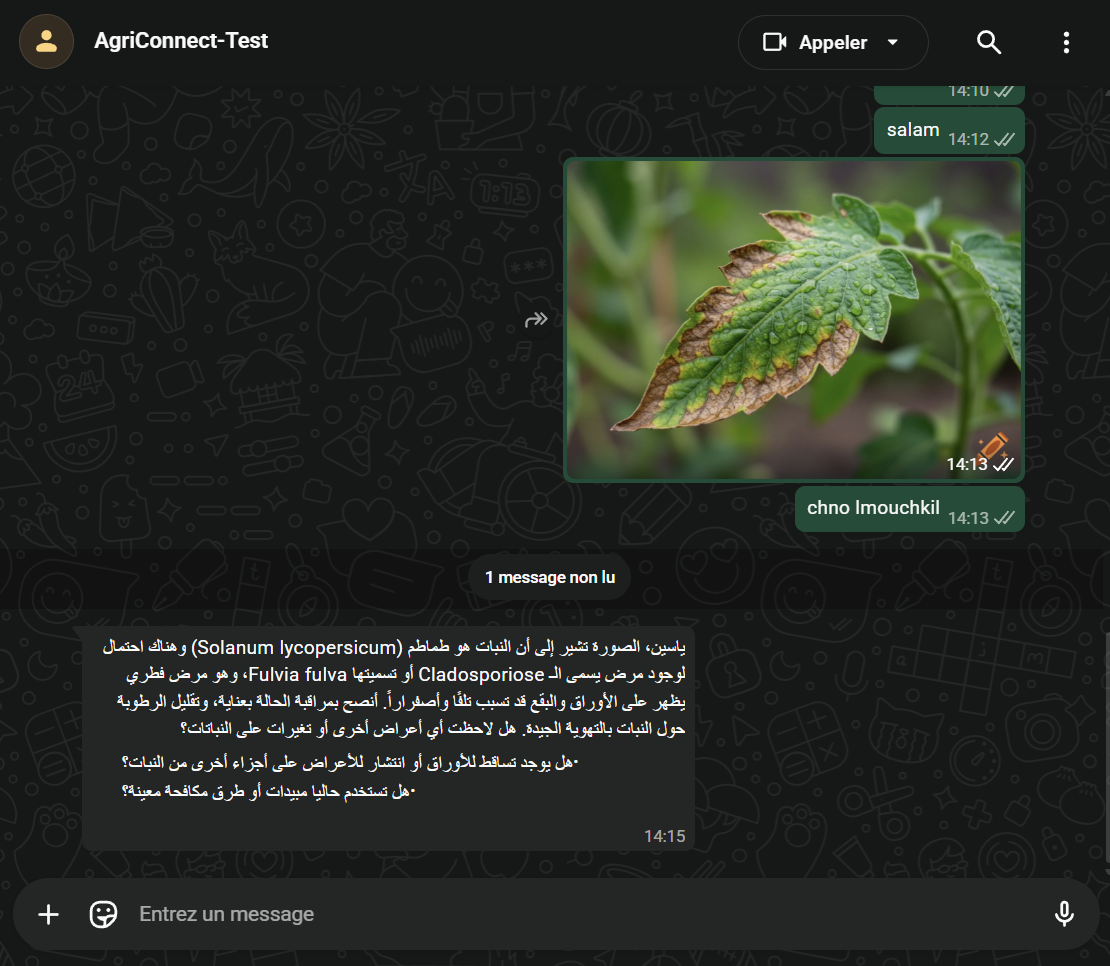
\includegraphics[width=0.55\textwidth]{images/results/scenario1_diagnosis_response.png}
\caption{WhatsApp conversation showing the farmer's crop image and the system's disease diagnosis response}
\label{fig:scenario1-whatsapp}
\end{figure}

\subsection{Scenario 2: Case Escalation to Agronomist}

A farmer sends three consecutive urgent text messages describing a rapidly spreading infestation across a wheat field. W00 buffers all three messages and W01 processes the full batch once idle. The Normalizer Agent detects a wheat crop, rapid leaf withering, and an explicit urgency signal. The Orchestrator Agent identifies the situation as high-urgency without sufficient image evidence and invokes the Escalation Agent, which creates a formal case in Supabase with status \textit{open} and priority \textit{medium}.

The farmer receives a WhatsApp notification confirming escalation to an agronomist. The case appears immediately in the agronomist interface with its priority level, farmer summary, crop photo, and location, as shown in Figures~\ref{fig:scenario2-whatsapp} and~\ref{fig:scenario2-case}.

\begin{figure}[H]
\centering

\includegraphics[width=0.55\textwidth]{images/results/scenario2_escalation_whatsapp.png}
\caption{WhatsApp notification sent to the farmer confirming case escalation to an agronomist}
\label{fig:scenario2-whatsapp}
\end{figure}

\begin{figure}[H]
\centering
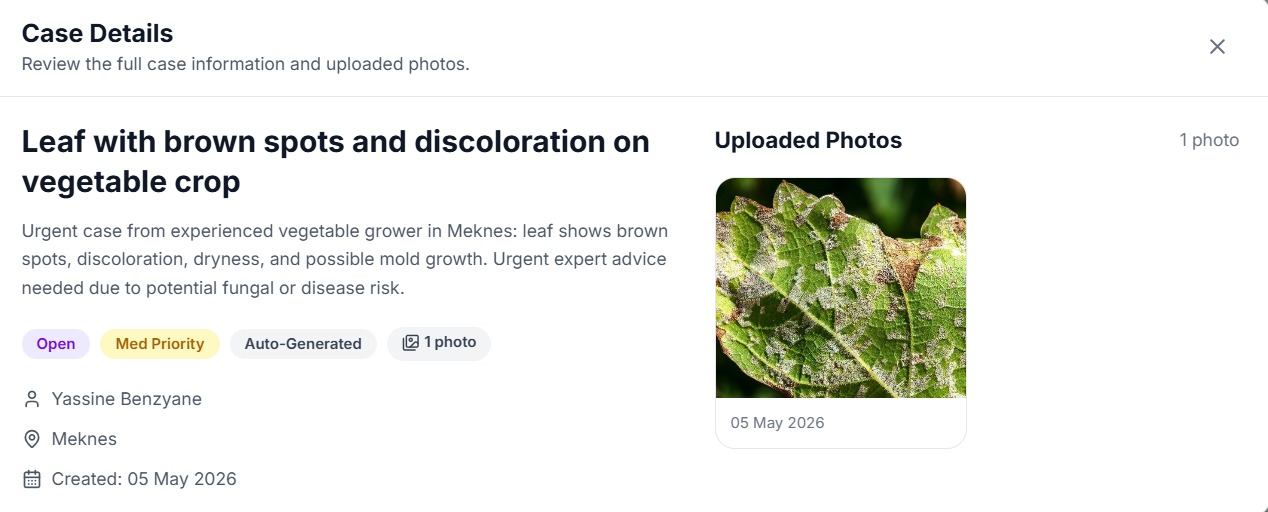
\includegraphics[width=0.9\textwidth]{images/results/scenario2_case_details.png}
\caption{Auto-generated case details visible in the agronomist interface, showing the crop image, case summary, priority, farmer name, and location}
\label{fig:scenario2-case}
\end{figure}

\section{Agent-Level Validation}

This section validates each specialized agent individually by presenting a controlled input and verifying that the structured output is semantically correct and conforms to the expected schema. For agents that produce a direct WhatsApp response visible to the farmer, the validation is illustrated through a screenshot of the resulting conversation. For the Normalizer Agent, which operates internally without producing a direct WhatsApp output, the structured JSON output is presented as a code excerpt.

\subsection{Normalizer Agent}

The Normalizer Agent is tested with a raw Redis buffer containing two messages in French: a text message describing yellow spots on tomato leaves and a reference to an attached image. The agent is expected to extract the farmer's main question in English, identify the crop and symptoms, detect the language, and produce a valid structured JSON object.

The output confirms that the agent correctly reformulated the question as \textit{"What disease is causing yellow spots on my tomato leaves?"}, identified the crop as tomato, extracted the symptoms as leaf discoloration and spotting, set the detected language to French, and reported no critical urgency signal. The Structured Output Parser validated the schema without errors. The resulting normalized object is shown below:

\begin{verbatim}
{
  "question_en": "What disease is causing yellow spots on my tomato leaves?",
  "detected_language": "fr",
  "summary": "Farmer reports yellow spots on tomato leaves.",
  "crop": "tomato",
  "symptoms": ["leaf discoloration", "spotting"],
  "urgency": false,
  "location_hint": null,
  "attachments": [{ "type": "image", "url": "farmers_media/images/..." }]
}
\end{verbatim}

\subsection{RAG Agent}

The RAG Agent is tested with a reformulated query asking about treatment methods for early blight on tomato crops. The agent is expected to perform a semantic search against the Supabase vector store and return the most relevant knowledge base chunks, which are then used to construct a grounded response.

The test confirms that the agent retrieved three relevant document chunks covering early blight identification criteria, recommended fungicide treatments, and preventive cultural practices. The response generated from these chunks is factually grounded and avoids unsupported claims, demonstrating that the retrieval mechanism correctly filters and prioritizes relevant content. Figure~\ref{fig:rag-whatsapp} shows the WhatsApp response delivered to the farmer, which visibly reflects the documented treatment recommendations retrieved from the knowledge base.

\begin{figure}[H]
\centering
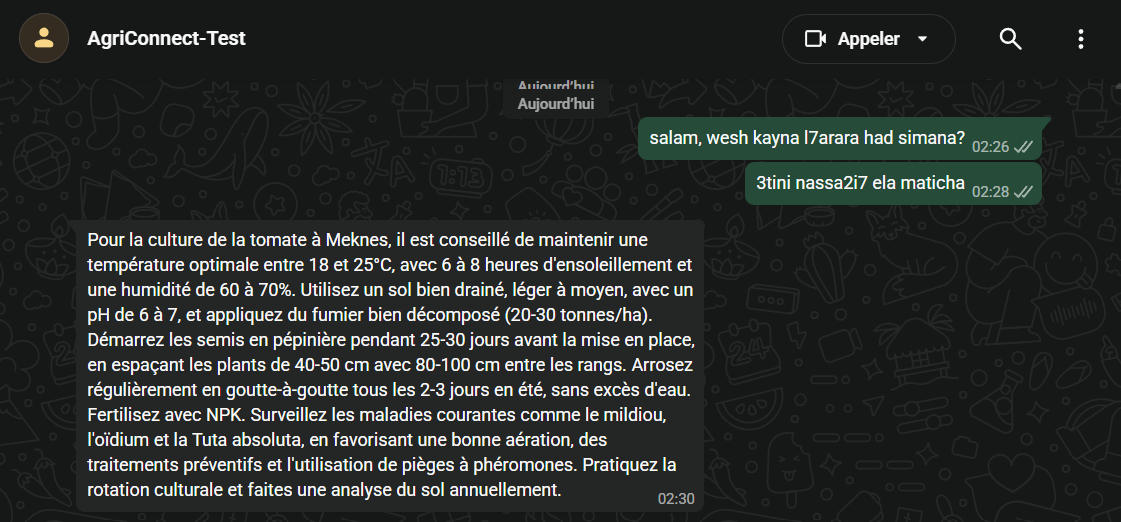
\includegraphics[width=0.55\textwidth]{images/results/rag_whatsapp_response.png}
\caption{WhatsApp response generated by the RAG Agent based on retrieved knowledge base passages}
\label{fig:rag-whatsapp}
\end{figure}

\subsection{Vision Agent}

The Vision Agent is tested by submitting a tomato leaf image showing yellow-brown spots with concentric rings to the Vision Sub-Workflow. The agent calls the four PlantNet endpoints in parallel and is expected to return a ranked list of disease candidates with confidence scores.

The results confirm that the disease identification endpoint returned \textit{Alternaria solani} (early blight) as the top candidate, with a confidence score consistent with the visible symptoms. The species identification endpoints confirmed the plant as \textit{Solanum lycopersicum} (tomato). The structured ensemble output included a recommended next step directing the orchestrator to invoke the RAG Agent for treatment retrieval. The WhatsApp response delivered to the farmer, shown in Figure~\ref{fig:vision-whatsapp}, reflects the plant identification result and the associated disease diagnosis.

\begin{figure}[H]
\centering
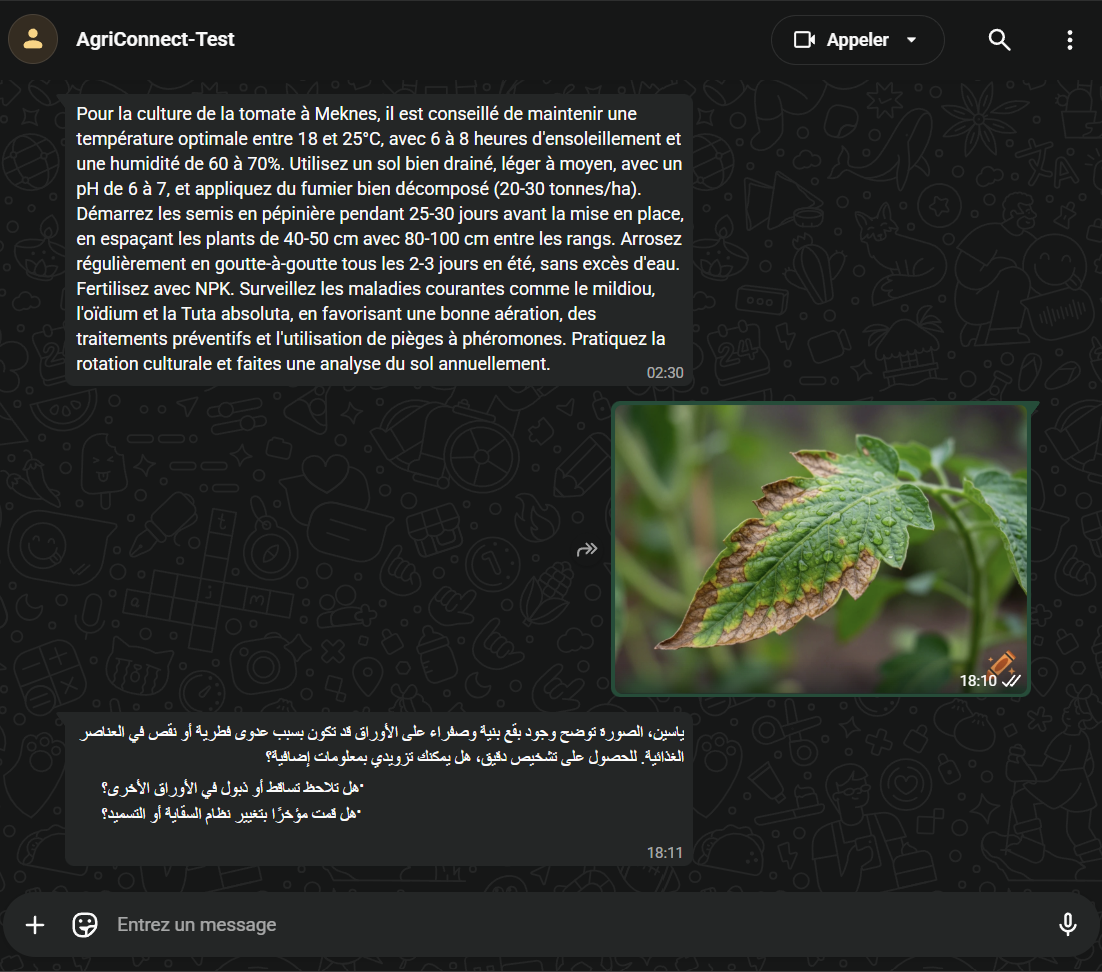
\includegraphics[width=0.55\textwidth]{images/results/vision_whatsapp_response.png}
\caption{WhatsApp response showing the Vision Agent's plant identification and disease diagnosis result}
\label{fig:vision-whatsapp}
\end{figure}

\subsection{Weather Agent}

The Weather Agent is tested using the coordinates of a registered farmer located in the Souss-Massa region. The agent is expected to query the weather API and return current meteorological conditions alongside agronomic signals relevant to the farmer's situation.

The output confirms that the agent retrieved current temperature, humidity, wind speed, and a five-day precipitation forecast. The synthesized agronomic signals indicated an elevated fungal disease risk window due to high humidity and upcoming rainfall, and flagged unfavorable spraying conditions for the following two days. These signals were correctly injected into the orchestrator's final response, which explicitly referenced the local weather context. Figure~\ref{fig:weather-whatsapp} shows the resulting WhatsApp message, where the recommendation is adapted to the farmer's current environmental conditions.

\begin{figure}[H]
\centering
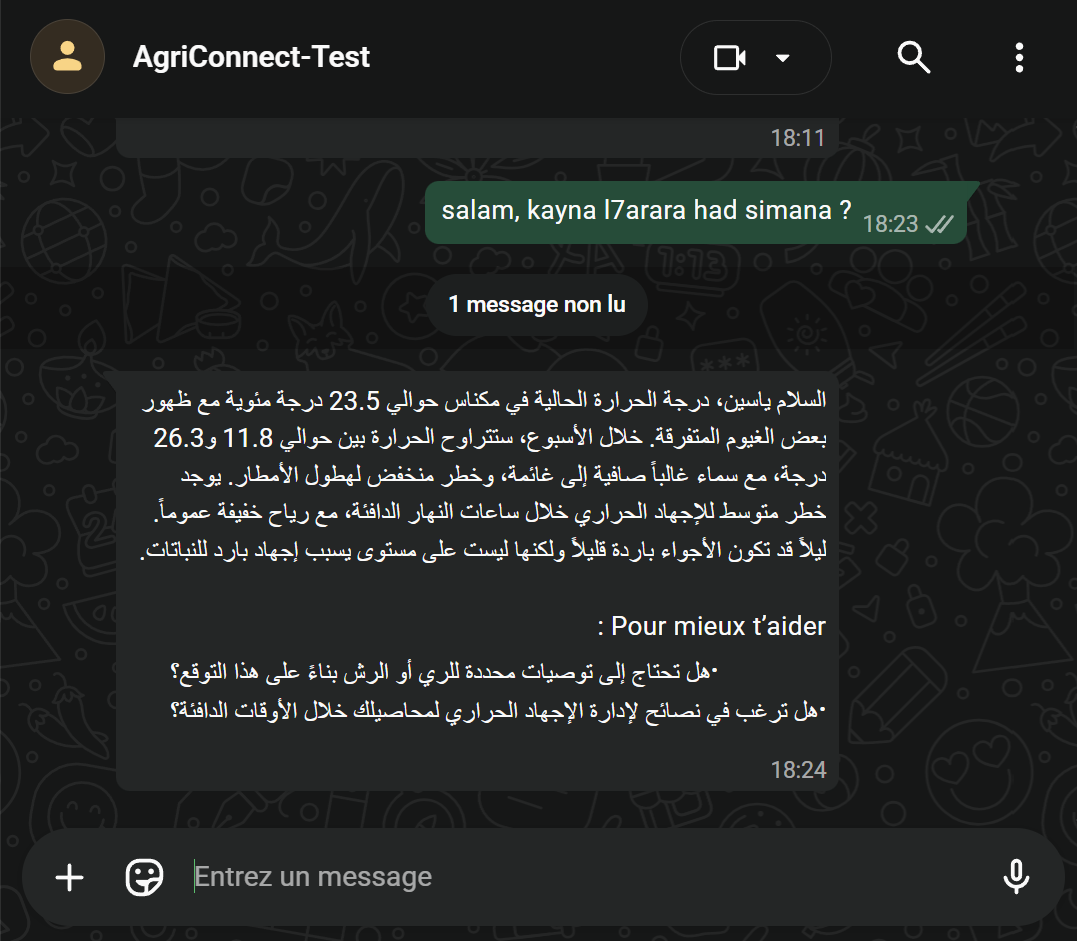
\includegraphics[width=0.55\textwidth]{images/results/weather_whatsapp_response.png}
\caption{WhatsApp response incorporating weather-aware agronomic advice from the Weather Agent}
\label{fig:weather-whatsapp}
\end{figure}

\subsection{Escalation Agent}

The Escalation Agent is tested by providing a normalized batch flagged as high-urgency with no eligible image for visual analysis. The agent is expected to create a formal case record in the Supabase database and make it immediately visible in the agronomist interface.

The test confirms that the agent created a case record with status \textit{open}, priority \textit{high}, and the correct farmer identifier. The farmer received an immediate WhatsApp notification informing them of the escalation, as illustrated in the end-to-end scenario presented in Figure~\ref{fig:scenario2-whatsapp}. The case appeared in the agronomist interface within seconds of the escalation trigger, as shown in Figure~\ref{fig:scenario2-case}.

\section{Web Application Testing}

This section presents the results of functional testing performed on the web application for each user role. Each use case is executed manually and recorded as passed or failed based on whether the expected behavior is observed in the interface and correctly reflected in the database.

\subsection{Farmer Interface}

Table~\ref{tab:farmer-tests} summarizes the functional test results for the farmer interface.

\begin{table}[H]
\centering
\caption{Functional test results — Farmer interface}
\label{tab:farmer-tests}
\begin{tabular}{p{6cm} p{5.5cm} c}
\toprule
\textbf{Use Case} & \textbf{Expected Behavior} & \textbf{Result} \\
\midrule
Register as farmer & Account created, redirected to dashboard & Pass \\
Login with credentials & Session initiated, role-based redirect & Pass \\
Create a new case with images & Case saved with images in Supabase & Pass \\
View case list by status & Cases grouped by open/assigned/resolved & Pass \\
Edit an open case & Case updated in database & Pass \\
Delete an open case & Case removed from list & Pass \\
View proposals on a case & Proposals modal displays correctly & Pass \\
Accept a proposal & Case status updated to assigned & Pass \\
Reject a proposal & Proposal marked as rejected & Pass \\
Provide feedback on resolved case & Feedback saved, case closed & Pass \\
View interactive map & Farmer and agronomist markers displayed & Pass \\
Update profile information & Profile updated in database & Pass \\
\bottomrule
\end{tabular}
\end{table}

\subsection{Agronomist Interface}

Table~\ref{tab:agronomist-tests} summarizes the functional test results for the agronomist interface.

\begin{table}[H]
\centering
\caption{Functional test results — Agronomist interface}
\label{tab:agronomist-tests}
\begin{tabular}{p{6cm} p{5.5cm} c}
\toprule
\textbf{Use Case} & \textbf{Expected Behavior} & \textbf{Result} \\
\midrule
Register with supporting documents & Account created with pending status & Pass \\
Login after admin approval & Access granted to agronomist dashboard & Pass \\
Browse open unassigned cases & Cases listed with details and images & Pass \\
Submit a proposal on a case & Proposal saved and visible to farmer & Pass \\
View accepted proposals & Cases moved to assigned section & Pass \\
Mark an assigned case as resolved & Case status updated to resolved & Pass \\
View intervention history & Past cases accessible in assigned section & Pass \\
Update profile and specialties & Profile updated in database & Pass \\
\bottomrule
\end{tabular}
\end{table}

\subsection{Administrator Interface}

Table~\ref{tab:admin-tests} summarizes the functional test results for the administrator dashboard.

\begin{table}[H]
\centering
\caption{Functional test results — Administrator interface}
\label{tab:admin-tests}
\begin{tabular}{p{6cm} p{5.5cm} c}
\toprule
\textbf{Use Case} & \textbf{Expected Behavior} & \textbf{Result} \\
\midrule
Login to admin dashboard & Access granted to admin interface & Pass \\
View platform statistics & Metrics and case distribution displayed & Pass \\
View all cases by status & Full case list accessible & Pass \\
Edit or delete any case & Changes reflected in database & Pass \\
Manage proposals and feedback & Edit and delete actions functional & Pass \\
Search users by name or email & Filtered results displayed correctly & Pass \\
Validate agronomist registration & Account status updated to approved & Pass \\
Reject agronomist registration & Account status updated to rejected & Pass \\
Deactivate a user account & Account access revoked & Pass \\
\bottomrule
\end{tabular}
\end{table}


\section{Discussion}

\subsection{Strengths of the System}

The evaluation results reveal several notable strengths in the AgriConnect platform that contribute to its practical relevance and technical soundness.

\textbf{Accessible interaction channel.} The choice of WhatsApp as the primary communication interface significantly lowers the adoption barrier for farmers. The system accepts text, audio, and image inputs without requiring farmers to install a dedicated application or navigate a formal web interface. This design choice is directly aligned with mobile usage patterns in rural Morocco~\cite{anrt2025}.

\textbf{Modular multi-agent architecture.} The separation of responsibilities across specialized agents ensures that each cognitive task is handled by a dedicated component. The orchestrator activates only the agents that are relevant to each specific request, which reduces unnecessary API calls, improves response latency for simple queries, and makes individual agents independently maintainable and replaceable.

\textbf{Knowledge-grounded responses.} The RAG Agent effectively grounds the system's agronomic recommendations in curated documentary evidence, significantly reducing the risk of hallucination compared to a purely generative approach. The retrieval results observed during testing demonstrated that the semantic search correctly prioritized the most relevant knowledge base passages across different query types~\cite{li2025llm}.

\textbf{Multimodal visual analysis.} The Vision Sub-Workflow's parallel submission to four PlantNet endpoints provides a more robust species and disease identification result than any single endpoint could offer. The ensemble output gives the orchestrator ranked candidates with confidence scores, enabling conservative and evidence-based response generation~\cite{zhu2025vlm}.

\textbf{Human-in-the-loop escalation.} The system correctly identifies situations that exceed its automated reasoning capacity and escalates them to agronomists without producing overconfident or potentially harmful responses. This design principle is essential for maintaining farmer trust and ensuring professional reliability in high-stakes agricultural decisions~\cite{yin2025foundation}.

\textbf{Weather-aware contextualization.} The integration of real-time meteorological data allows the system to produce localized and operationally relevant recommendations. Agronomic advice that accounts for upcoming weather conditions is more actionable than generic guidance, particularly for decisions related to treatment timing, irrigation, and disease risk management~\cite{worldbank2024irrigation}.

\textbf{Role-based web application.} All functional tests across the farmer, agronomist, and administrator interfaces passed successfully, confirming that the web application correctly enforces role-based access, maintains data consistency, and supports the full case lifecycle from creation to closure.

\subsection{Identified Limitations}

Despite the positive evaluation results, several limitations were identified during testing that constrain the current performance and scope of the platform.

\textbf{PlantNet coverage of Moroccan crops.} The PlantNet API is trained on globally distributed botanical datasets and may not achieve optimal accuracy for crop varieties and disease manifestations specific to the Moroccan agricultural context. In particular, visual symptoms caused by drought stress, salinity, or nutrient deficiencies common in Moroccan fields may be misclassified as pathological disorders.

\textbf{Limited Darija language support.} Although the Normalizer Agent demonstrated robust handling of French and standard Arabic inputs, support for Darija, the Moroccan colloquial dialect most commonly used by rural farmers, depends entirely on the underlying language model's training data. The accuracy of normalization and question reformulation may degrade for heavily dialectal or mixed-language messages.

\textbf{Image quality dependency.} The Vision Agent's performance is sensitive to image quality. Images captured in poor lighting conditions, at suboptimal angles, or with partial crop coverage may fail the preanalysis quality gate or yield unreliable PlantNet results. In real field conditions, farmers may not always be able to provide optimal images.

\textbf{Fixed inactivity buffer window.} The Redis-based buffering mechanism relies on a fixed inactivity TTL to determine when a farmer has finished sending messages. This window may be too short for farmers who send messages slowly or in multiple sessions, potentially triggering premature batch processing before all messages have been received.

\textbf{Knowledge base scope and maintenance.} The quality of RAG-based responses depends directly on the content and coverage of the knowledge base. If a farmer's query concerns a crop or condition not covered by any ingested document, the RAG Agent cannot retrieve relevant evidence and the orchestrator must fall back to general language model knowledge, which carries a higher hallucination risk.

\textbf{Dependency on farmer location data.} The Weather Agent requires the farmer's geographical coordinates to retrieve localized meteorological data. If the farmer has not provided a location in their profile, weather-aware reasoning cannot be performed, which limits the system's ability to contextualize recommendations for farmers with incomplete profiles.

\textbf{Scalability of the polling mechanism.} The W01 orchestrator workflow runs on a five-second polling schedule, scanning all active Redis buffer keys on each execution. While this approach is effective at low to moderate load, it may introduce performance bottlenecks as the number of concurrent active farmers increases, since each polling cycle must inspect all active buffers before identifying ready ones.

\section{Chapter Summary}

This chapter presented a comprehensive evaluation of the AgriConnect platform through three complementary levels of testing: end-to-end scenario walkthroughs, agent-level validation, and functional testing of the web application.

The two end-to-end scenarios demonstrated that the full pipeline operates correctly in realistic conditions, from WhatsApp message reception to response delivery, covering both the multimodal disease diagnosis flow and the case escalation flow. The agent-level validation confirmed that each specialized agent — Normalizer, RAG, Vision, Weather, and Escalation — produces structured and semantically correct outputs for controlled inputs. The functional test tables showed that all key use cases across the farmer, agronomist, and administrator interfaces passed successfully.

The discussion highlighted the system's main strengths, including its accessible WhatsApp interface, modular multi-agent architecture, knowledge-grounded responses, and effective human-in-the-loop escalation. It also identified several current limitations related to Moroccan crop coverage, Darija language handling, image quality sensitivity, and knowledge base maintenance.

Overall, the evaluation confirms that AgriConnect fulfills its core requirements and demonstrates the feasibility of an integrated, multimodal, and knowledge-grounded agricultural assistance platform adapted to the Moroccan context. The identified limitations provide a clear basis for future improvements, which are discussed in the conclusion chapter.
